\documentclass[11pt,a4paper]{article}
\usepackage[margin=1in]{geometry}
\usepackage[T1]{fontenc}
\usepackage{lmodern}
\usepackage{parskip}
\usepackage[hidelinks]{hyperref}
\usepackage{tabularx}
\usepackage{booktabs}
\usepackage{xcolor}
\usepackage{enumitem}
\usepackage{microtype}
\usepackage{float}

% TikZ + scaling helper for the diagram
\usepackage{tikz}
\usetikzlibrary{arrows.meta,positioning,calc,fit,matrix}
\usepackage{adjustbox}

\setlist{itemsep=0.25em, topsep=0.25em}
\hypersetup{colorlinks=true,linkcolor=black,urlcolor=blue}

\begin{document}

\begin{center}
    \Large \textbf{Synopsis of Data Structures Lab PBL} \\
    \vspace{0.5cm}
    \large \textbf{Terminal Data Structures \& Algorithms Visualizer} \\
    \vspace{0.5cm}
\end{center}

\noindent
\textbf{Department:} Department of Computer Science \& IT \\
\textbf{Faculty Guide:} 
\begin{itemize}[nosep,left=0pt]
    \item Dr. Anupama Padha
    \item Dr. Dhanalekshmi G
\end{itemize}

\noindent
\textbf{Group Members:}
\begin{itemize}[nosep,left=0pt]
    \item Harsh Sharma (2401030232)
    \item Karvy Singh (2401030234)
    \item Rudra Kumar Singh (2401030237)
\end{itemize}

\noindent
\textbf{Batch:} B5


\section*{Brief Description}
\textbf{Terminal Data Structures \& Algorithms Visualizer} is a text-based tool that shows how common data structures and algorithms work, directly in the terminal. It uses simple block characters and a little color to animate each step. The goal is to make the logic easy to understand and to let students see what happens during inserts, searches, swaps, rotations, and probes.

\subsection*{Main Features}
\begin{itemize}[nosep]
  \item \textbf{Sorting animations:} Bubble, Insertion, Selection, Merge, Quick, and Heap sort. Bars move and swap so we can follow every comparison.
  \item \textbf{Hash map demo:} Insert/search/delete with four collision methods: \emph{separate chaining}, \emph{linear probing}, \emph{quadratic probing}, and \emph{double hashing}. We show probe paths and load factor.
  \item \textbf{Trees \& heaps:} Binary Search Tree (BST), AVL (with rotations), and Binary Heap (min/max).
  \item \textbf{Graphs:} BFS and DFS on a small graph (adjacency list).
  \item \textbf{Controls:} Play/pause, single-step, speed, input size, random or custom inputs, fixed seed for repeatable runs.
\end{itemize}

\section*{Mapping to Real-Life Applications}
\begin{tabularx}{\textwidth}{@{}p{35mm}X@{}}
\toprule
\textbf{Topic} & \textbf{Where it shows up} \\
\midrule
Sorting (Quick/Merge/Heap) & Ordering rows in databases, cleaning logs, ranking search results. \\
Hash Map (Chaining/Probing) & Very fast key--value lookups: caches, symbol tables in compilers, routing tables. \\
BST / AVL & In-memory indexes and range queries with predictable $O(\log n)$ time. \\
Binary Heap (PQ) & Schedulers and priority queues; Dijkstra/A* shortest path. \\
Graphs (BFS/DFS) & Network reachability, crawling web pages, finding connections in social graphs. \\
\bottomrule
\end{tabularx}

\section*{Data Structures \& Algorithms (Class Diagram)}
% ===================== REPLACE YOUR FIGURE WITH THIS =====================
\begin{figure}[H]
\centering
\setlength{\abovecaptionskip}{4pt}

% ================= (A) Sorting + Core DS & Graph Algorithms (TOP) =================
{\large\textbf{(A) Sorting + Core DS \& Graph Algorithms}}\par\vspace{0.4em}
\begin{adjustbox}{max width=.98\linewidth}
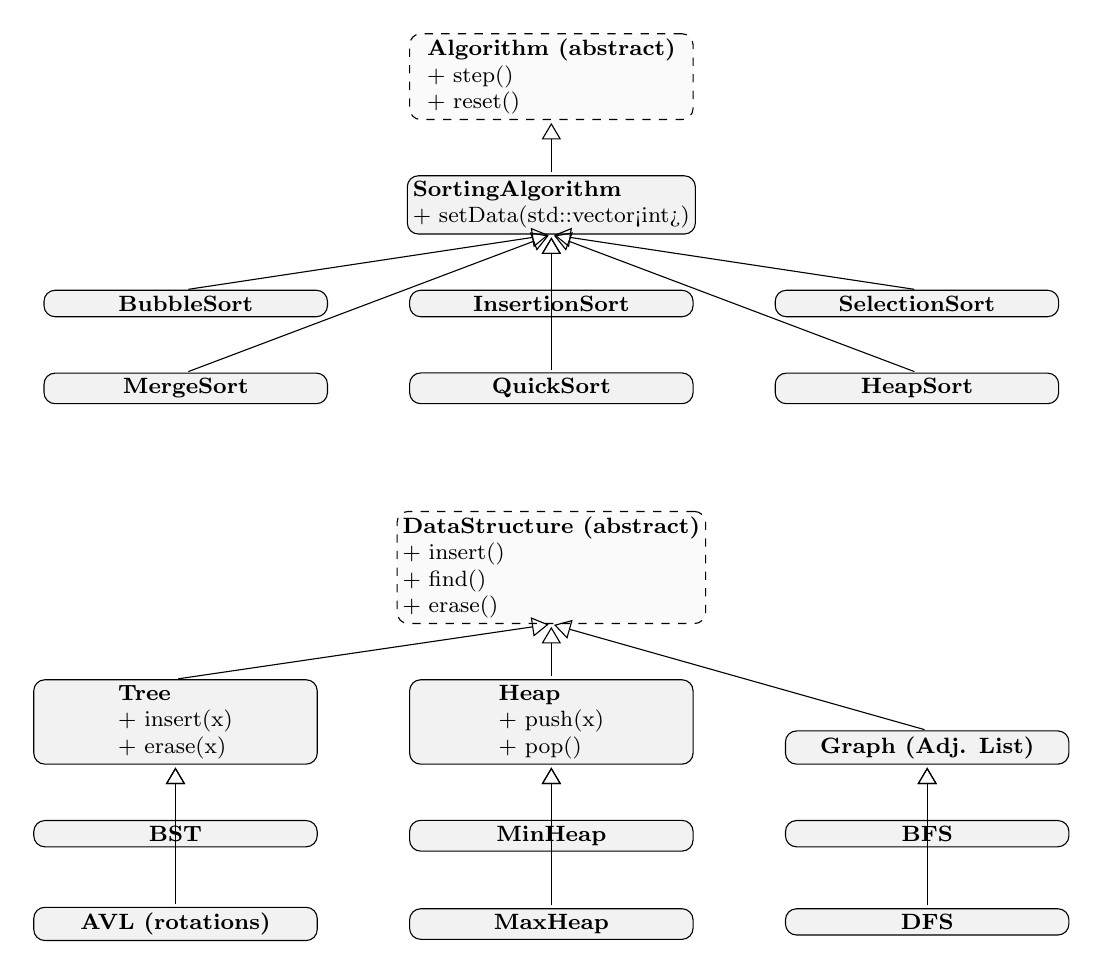
\begin{tikzpicture}[
  >=Stealth,
  every node/.style={inner sep=2pt},
  box/.style={draw, rounded corners, fill=gray!10, align=left, minimum width=36mm, font=\footnotesize},
  abox/.style={draw, rounded corners, fill=gray!4,  align=left, minimum width=36mm, font=\footnotesize, dashed},
  inh/.style={-{Triangle[open,width=7pt,length=6pt]}, shorten >=1pt, shorten <=1pt},
  row sep=7mm, column sep=10mm
]

% --- Sorting cluster (parents centered) ---
\matrix (sort) [matrix of nodes] {
  \node{}; & \node[abox] (alg) {\textbf{Algorithm (abstract)}\\ + step()\\ + reset()}; & \node{}; \\
  \node{}; & \node[box]  (salg) {\textbf{SortingAlgorithm}\\ + setData(std::vector<int>)}; & \node{}; \\
  \node[box] (bubble) {\textbf{BubbleSort}}; &
  \node[box] (insert) {\textbf{InsertionSort}}; &
  \node[box] (select) {\textbf{SelectionSort}}; \\
  \node[box] (merge)  {\textbf{MergeSort}}; &
  \node[box] (quick)  {\textbf{QuickSort}}; &
  \node[box] (heap)   {\textbf{HeapSort}}; \\
};
\draw[inh] (salg.north) -- (alg.south);
\foreach \n in {bubble,insert,select,merge,quick,heap} {
  \draw[inh] (\n.north) -- (salg.south);
}

% --- Core DS in 3 columns (parents centered, vertical edges only) ---
\matrix (core) [matrix of nodes, below=12mm of sort] {
  \node{}; & \node[abox] (dsabs) {\textbf{DataStructure (abstract)}\\ + insert()\\ + find()\\ + erase()}; & \node{}; \\
  \node[box]  (tree)  {\textbf{Tree}\\ + insert(x)\\ + erase(x)}; &
  \node[box]  (heapds){\textbf{Heap}\\ + push(x)\\ + pop()}; &
  \node[box]  (graph) {\textbf{Graph (Adj. List)}}; \\
  \node[box]  (bst)   {\textbf{BST}}; &
  \node[box]  (minhp) {\textbf{MinHeap}}; &
  \node[box]  (bfs)   {\textbf{BFS}}; \\
  \node[box]  (avl)   {\textbf{AVL (rotations)}}; &
  \node[box]  (maxhp) {\textbf{MaxHeap}}; &
  \node[box]  (dfs)   {\textbf{DFS}}; \\
};
% parents to abstract
\draw[inh] (tree.north)   -- (dsabs.south);
\draw[inh] (heapds.north) -- (dsabs.south);
\draw[inh] (graph.north)  -- (dsabs.south);
% children straight under parents
\draw[inh] (bst.north)    -- (tree.south);
\draw[inh] (avl.north)    -- (tree.south);
\draw[inh] (minhp.north)  -- (heapds.south);
\draw[inh] (maxhp.north)  -- (heapds.south);
\draw[inh] (bfs.north)    -- (graph.south);
\draw[inh] (dfs.north)    -- (graph.south);

\end{tikzpicture}
\end{adjustbox}

\vspace{0.9em}

% ================= (B) Hash Map + Collision Strategies (BOTTOM) =================
{\large\textbf{(B) Hash Map \& Collision Strategies}}\par\vspace{0.4em}
\begin{adjustbox}{max width=.98\linewidth}
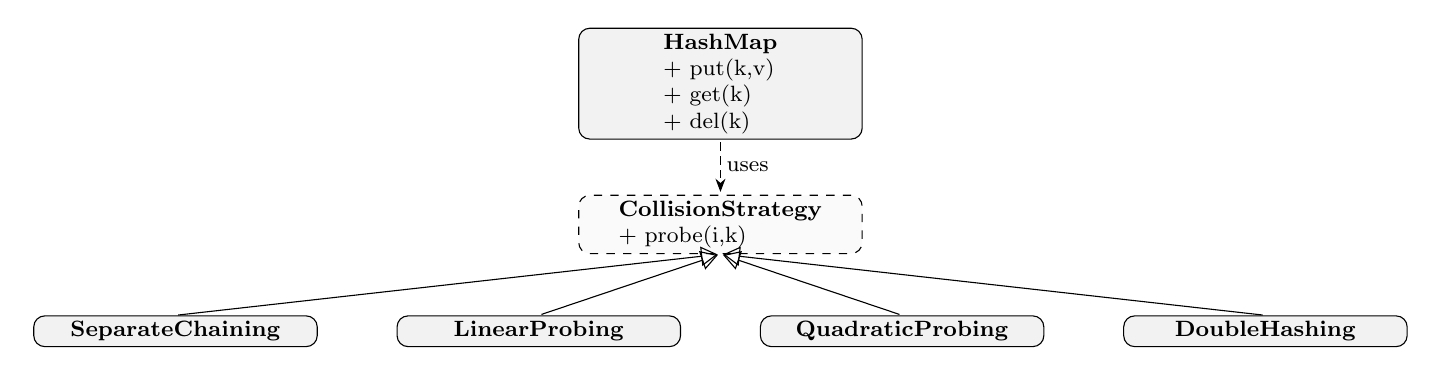
\begin{tikzpicture}[
  >=Stealth,
  every node/.style={inner sep=2pt},
  box/.style={draw, rounded corners, fill=gray!10, align=left, minimum width=36mm, font=\footnotesize},
  abox/.style={draw, rounded corners, fill=gray!4,  align=left, minimum width=36mm, font=\footnotesize, dashed},
  inh/.style={-{Triangle[open,width=7pt,length=6pt]}, shorten >=1pt, shorten <=1pt},
  uses/.style={densely dashed, -Stealth, shorten >=1pt, shorten <=1pt},
  node distance=7mm and 10mm,
  row sep=7mm, column sep=10mm
]

% Parents centered (no matrix so they sit exactly on the center)
\node[box]  (hmap) {\textbf{HashMap}\\ + put(k,v)\\ + get(k)\\ + del(k)};
\node[abox, below=7mm of hmap] (cabs) {\textbf{CollisionStrategy}\\ + probe(i,k)};

% Children in a separate 4-column row, centered under the strategy
\matrix (kids) [matrix of nodes, below=7mm of cabs, column sep=10mm] {
  \node[box] (chain) {\textbf{SeparateChaining}}; &
  \node[box] (lin)   {\textbf{LinearProbing}}; &
  \node[box] (quad)  {\textbf{QuadraticProbing}}; &
  \node[box] (dh)    {\textbf{DoubleHashing}}; \\
};

% Short vertical 'uses' edge
\draw[uses] (hmap.south) -- node[right, font=\footnotesize]{uses} (cabs.north);

% Two ports on the strategy's south edge to fan-in arrows cleanly
\coordinate (portL) at ([xshift=6mm]cabs.south west);
\coordinate (portR) at ([xshift=-6mm]cabs.south east);

\draw[inh] (chain.north)  -- (cabs.south);
\draw[inh] (lin.north)    -- (cabs.south);
\draw[inh] (quad.north)   -- (cabs.south);
\draw[inh] (dh.north)     -- (cabs.south);

\end{tikzpicture}
\end{adjustbox}

% \caption{Top: sorting and core data structures/graph algorithms. Bottom: hash map and collision strategies. Parents are centered; inheritance lines are vertical or orthogonal for tidy layout.}
\end{figure}
% ===================== END REPLACEMENT =====================


\end{document}
